 \documentclass[a4paper,10pt]{article}
\input{/Users/WannaGetHigh/workspace/latex/macros.tex}

\title{Rapport TP2 : SMA - Billes / Shelling / proies-pr\'edateurs }
\author{Fran\c{c}ois \bsc{Lepan} - Alexis \bsc{Linke}}

\begin{document}
\maketitle

\section{Choix}

Nous sommes partis sur un syst\`eme de d\'eplacement sur une grille case par case. Deux agents ne peuvent  se retrouver sur une m\^eme case.

Nous avons fait ce choix car le syst\`eme de collision ainsi que la repr\'esentation sur un \verb&JPanel& est plus facile \`a g\'erer qu'un syst\`eme de d\'eplacement libre.

Les couleurs des Billes sont fix\'es lors de leurs cr\'eation. \\

Pour repr\'esenter le mod\`ele de Schelling nous avons choisi une population divis\'ee en deux type : la population bleue et la population jaune, d'\'egale importance. Chaque membre peut regarder dans le voisinage de Moore pour estimer son niveau de satisfaction et s'il n'est pas satisfait il se t\'el\'eporte al\'eatoirement dans l'environnement. Un fichier \emph{Schelling.txt} est cr\'e\'e lors de l'ex\'ecution du code donnant le taux de satisfaction sur la dur\'ee de la simulation. \\

Pour le mod\`ele proies - pr\'edateur nous avons avons choisis de cr\'eer deux sous classe de Agent l'un pour les proies et l'autre pour les pr\'edateurs. Les positions ainsi que les directions sont d\'efini al\'eatoirement lors de la cr\'eation de ces deux Agents. L'environnement de d\'eplacement est torique.
Deux fichier sont cr\'eer lors de la simulation : \\

\begin{itemize}
\item \emph{ages\_prey\_pred.txt} : contenant les ages de tous les agents \`a chaque tour de simulation.
\item \emph{population\_prey\_pred.txt} : contenant le nombre de proie et de pr\'edateur \`a chaque tour de simulation.
\end{itemize}
\newpage

\section{UML}

\begin{figure}[ht]
\begin{center}
	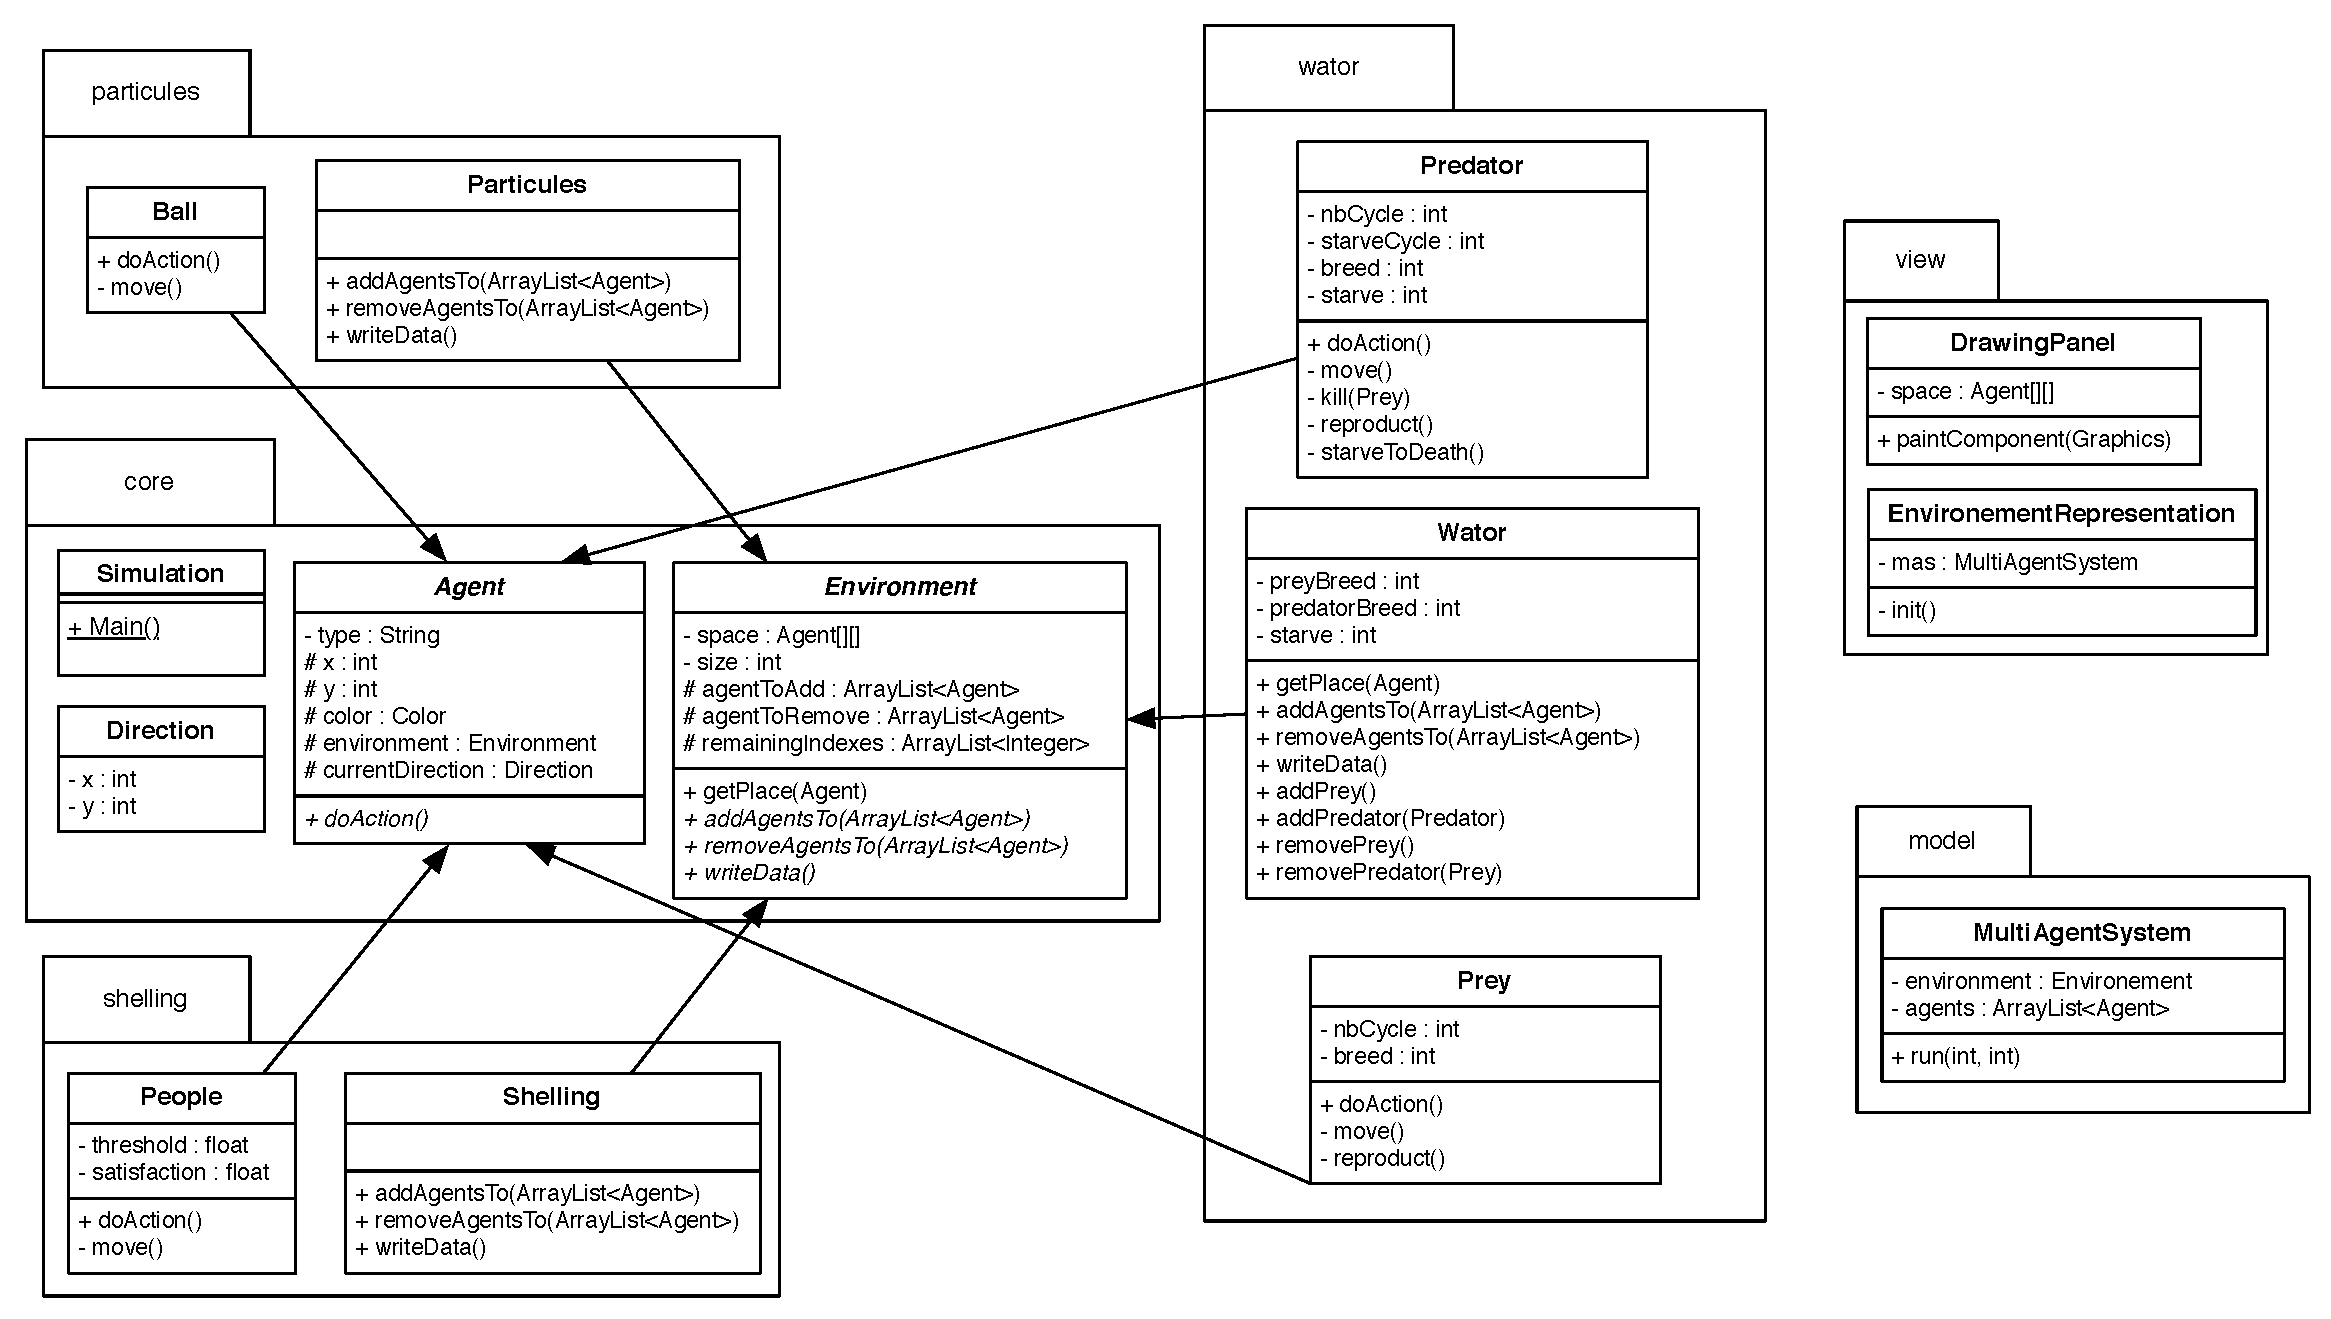
\includegraphics[width=15cm]{uml/sci_uml_tp2.pdf}
\end{center}
	\caption{UML}
	\label{uml}
\end{figure}

\section{Compilation + fonctionnement}
 
\paragraph{Compilation} ~\\
Se mettre dans le dossier src $\rightarrow$ \verb&javac core/Simulation.java&

\paragraph{Execution} ~\\
Ne pas bouger du dossier src \\
Si on rentre un nombre de tour = -1 alors c'est infini \\

Pour la Simulation des Billes : \\ 
\verb&java core.Simulation -b <taille> <nb agent> <nb tour> <delai entre chaque tour>& \\

Pour la Simulation du mod\`ele de Shelling : \\ 
\verb&java core.Simulation -s <taille> <nb habitant> <seuil tolerance> <nb tour> <delai>& \\
Avec le seuil de tol\'erance compris entre 0 et 1. \\

Pour la Simulation du mod\`ele de Proies - P\'edateur : \\ 
\verb&java core.Simulation -w <taille> <nb proies> <nb pred> <tps reprod proies> <tps reprod pred>&
 \verb&<tps faim> <delai>& \\

\paragraph{Exemples} ~\\

Billes : \\
~
\verb&java core.Simulation -b 100 50 -1 5& \\
\verb&java core.Simulation -b 10 5 100 5& \\
\verb&java core.Simulation -b 50 40 -1 5& \\

Shelling : \\
~
\verb&java core.Simulation -s 100 9750 0.3 -1 1& \\
\verb&java core.Simulation -s 100 9750 0.6 -1 1 & \\
\verb&java core.Simulation -s 50 2000 0.7 -1 100 & \\

Proies-Pr\'edateurs : \\
~
\verb&java core.Simulation -w 50 1040 326 4 10 6 -1 50& \\
\verb&java core.Simulation -w 10 10 5 4 10 6 -1 50& \\
\verb&java core.Simulation -w 35 100 30 4 10 6 -1 50& \\

\section{Probl\`eme}

Nous avons un probl\`eme pour le redimensionnement de la fen\`etre, il y a un e\'cart qui se forme en bas et \`a droite de cette fen\`etre.

Pour Shelling lorsque le seuil est de 0.8 ou plus, la population ne se stabilise pas.

Pour le mod\`ele proies - pr\'edateurs il y a un probl\`eme sur l'\'evolution de la population. Certain agents vives beaucoup trop longtemps. 
\end{document}